\documentclass[tikz, border=5pt]{standalone}
%\usepackage[utf8]{inputenc}
%\usepackage[spanish]{babel}
\usepackage{tikz}
\usetikzlibrary{matrix, backgrounds, arrows, decorations.markings}
\begin{document}
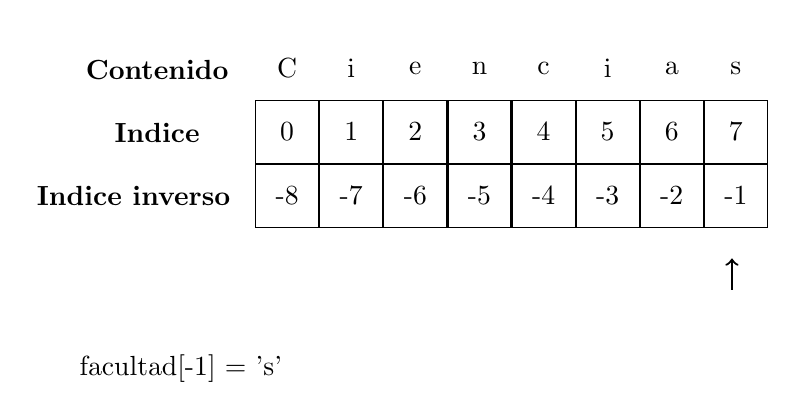
\begin{tikzpicture}
\node at (-4.5, 0.8) {$\textbf{Contenido}$};
\node at (-4.5, 0) {$\textbf{Indice}$};
\node at (-4.8, -0.8) {$\textbf{Indice inverso}$};
\draw [->, thick] (2.8, -2) -- (2.8, -1.6);
\matrix (m) [matrix of nodes,
             nodes={draw, minimum size=8mm,anchor=center},
             nodes in empty cells, minimum height = 1cm,
             row 1/.style={nodes={draw=none}},]
{
  C & i & e & n & c & i & a & s  \\
  0 & 1 & 2 & 3 & 4 & 5 & 6 & 7 \\
  -8 & -7 & -6 & -5 & -4 & -3 & -2 & -1 \\
};
\node at (-4.2, -3) {facultad[-1] = 's'};
\end{tikzpicture}
\end{document}